\section{1971 --- Find if Path Exists in Graph (LeetCode)}

\subsection*{Código}
\lstinputlisting{1971_FindIfPathExists.java}

\subsection*{Comprovante de aceite}
\begin{center}
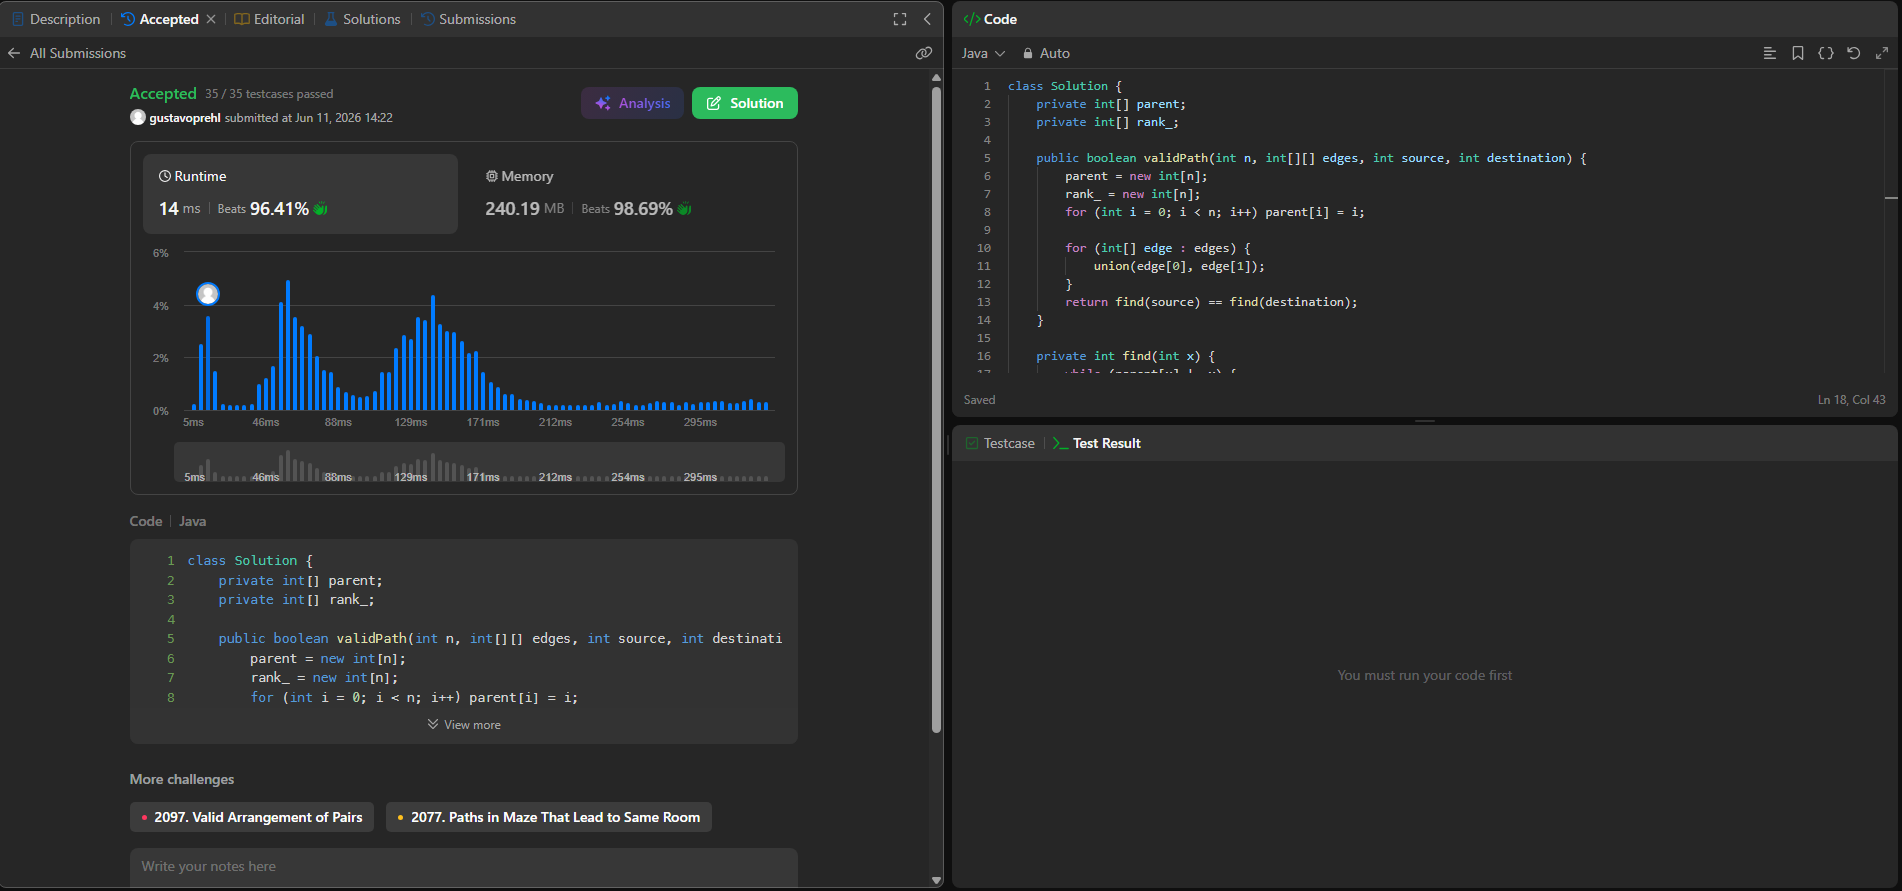
\includegraphics[width=0.85\textwidth]{Accepts/1971_FindIfPathExists_Submit.png}\\
\end{center}

\subsection*{Justificativa}

\textbf{Estratégia:} Union-Find (\emph{Disjoint Set Union} --- DSU) com
compressão de caminho e união por \emph{rank}.

\textbf{Modelagem:} existe um caminho entre \texttt{source} e
\texttt{destination} se e somente se os dois vértices pertencem ao mesmo
componente conexo do grafo. A estrutura DSU mantém uma partição dos vértices
em conjuntos disjuntos, onde cada conjunto representa um componente conexo,
identificado por um representante (raiz).

\textbf{Construção:} inicialmente cada vértice é seu próprio conjunto
(\texttt{parent[i] = i}). Para cada aresta \texttt{(u, v)} em \texttt{edges},
executa-se \texttt{union(u, v)}, unindo os conjuntos aos quais \texttt{u} e
\texttt{v} pertencem. Ao final, basta verificar se
\texttt{find(source) == find(destination)}.

\textbf{Compressão de caminho (\texttt{find}):} ao buscar a raiz de um
elemento, cada nó visitado é reconectado mais perto da raiz (aqui via
\emph{path halving}: \texttt{parent[x] = parent[parent[x]]}), achatando a
árvore e acelerando buscas futuras.

\textbf{União por rank (\texttt{union}):} ao unir dois conjuntos, a raiz da
árvore de menor \texttt{rank} (altura estimada) é pendurada na raiz da árvore
de maior \texttt{rank}, evitando que as árvores fiquem muito altas.

\textbf{Complexidade (teoria de DSU):} combinando compressão de caminho e
união por rank, cada operação \texttt{find}/\texttt{union} tem custo
amortizado $O(\alpha(n))$, onde $\alpha$ é a inversa da função de Ackermann
--- na prática, uma constante muito pequena ($\leq 4$ para qualquer $n$
razoável).

\begin{itemize}
    \item Tempo: $O((n + |edges|) \cdot \alpha(n)) \approx O(n + |edges|)$.
    \item Espaço: $O(n)$ para os vetores \texttt{parent} e
    \texttt{rank\_}.
\end{itemize}

\textbf{Tópico do curso:} a construção do DSU é puramente iterativa (laços
sobre os vértices e sobre \texttt{edges}), enquadrando-se em \emph{Análise de
Algoritmos Iterativos} [CLRS09, caps. 1 e 2.2]; como o tempo total é
quase-linear, $O((n+|edges|)\cdot\alpha(n))$, o algoritmo também é um exemplo
de problema na \emph{Classe P} [CLRS09, cap. 34.1].
